\documentclass[tikz,border=6pt]{standalone}
\usepackage{amsmath,amssymb,mathtools,physics,bm,nicefrac,wasysym}
\usepackage{xcolor}

\definecolor{colone}{RGB}{180,60,60}
\definecolor{coltwo}{RGB}{60,110,180}
\definecolor{colthree}{RGB}{60,140,80}

\definecolor{accent}{HTML}{A13D2C}
\definecolor{accent2}{HTML}{2B5F6B}
\definecolor{muted}{HTML}{5A564F}
\definecolor{panel}{HTML}{F8F6F0}
\definecolor{linecol}{HTML}{D8D2C4}
\definecolor{ink}{HTML}{1E1C1A}
\definecolor{astroblue}{HTML}{1B4F72}
\definecolor{astrodark}{HTML}{17202A}
\definecolor{sunyellow}{HTML}{E8A33D}

\usetikzlibrary{calc,arrows.meta,positioning,decorations.pathreplacing,decorations.markings,angles,quotes,shapes.geometric}
\usepackage{tikz-3dplot}

\newcommand{\vecr}{\vec r}
\newcommand{\vecL}{\vec L}
\newcommand{\vecA}{\vec A}
\newcommand{\vecf}{\vec f}
\newcommand{\vecF}{\vec F}
\newcommand{\vecp}{\vec p}
\newcommand{\avg}[1]{\left\langle #1\right\rangle}
\newcommand{\vecx}{\vec x}
\newcommand{\hatn}{\hat n}
\newcommand{\rhat}{\hat r}
\newcommand{\phihat}{\hat\phi}
\newcommand{\thetahat}{\hat\theta}
\newcommand{\note}[1]{\textcolor{blue!60!black}{\textit{[#1]}}}

% Astronomical acronyms
\newcommand{\LST}{\mathrm{LST}}
\newcommand{\GST}{\mathrm{GST}}
\newcommand{\GMST}{\mathrm{GMST}}
\newcommand{\GAST}{\mathrm{GAST}}
\newcommand{\LMST}{\mathrm{LMST}}
\newcommand{\LAST}{\mathrm{LAST}}
\newcommand{\UT}{\mathrm{UT}}
\newcommand{\UTC}{\mathrm{UTC}}
\newcommand{\TAI}{\mathrm{TAI}}
\newcommand{\TT}{\mathrm{TT}}
\newcommand{\TDB}{\mathrm{TDB}}
\newcommand{\JD}{\mathrm{JD}}
\newcommand{\MJD}{\mathrm{MJD}}
\newcommand{\EoT}{\mathrm{EoT}}
\newcommand{\SNR}{\mathrm{SNR}}
\newcommand{\RON}{\mathrm{RON}}

% Helper commands for specific diagrams
\newcommand{\midlinelabel}[3]{
    \node (midlabel) at ($ (#1)!.5!(#2) $) {#3};
    \draw[stealth-] (#1) --  (midlabel);
    \draw[-stealth] (midlabel) -- (#2);
}
\newcommand{\midlinelabell}[3]{
    \node[fill = white, inner sep = 0.2pt, outer sep=3pt] (midlabel) at ($ (#1)!.5!(#2) $) {#3};
    \draw[stealth-] (#1) --  (midlabel);
    \draw[-stealth] (midlabel) -- (#2);
}
\newcommand{\midlinelabelll}[3]{
    \node[fill = white, inner sep = 0.2pt, outer sep=3pt,scale=0.6] (midlabel) at ($ (#1)!.5!(#2) $) {#3};
    \draw[stealth-] (#1) --  (midlabel);
    \draw[-stealth] (midlabel) -- (#2);
}



\begin{document}
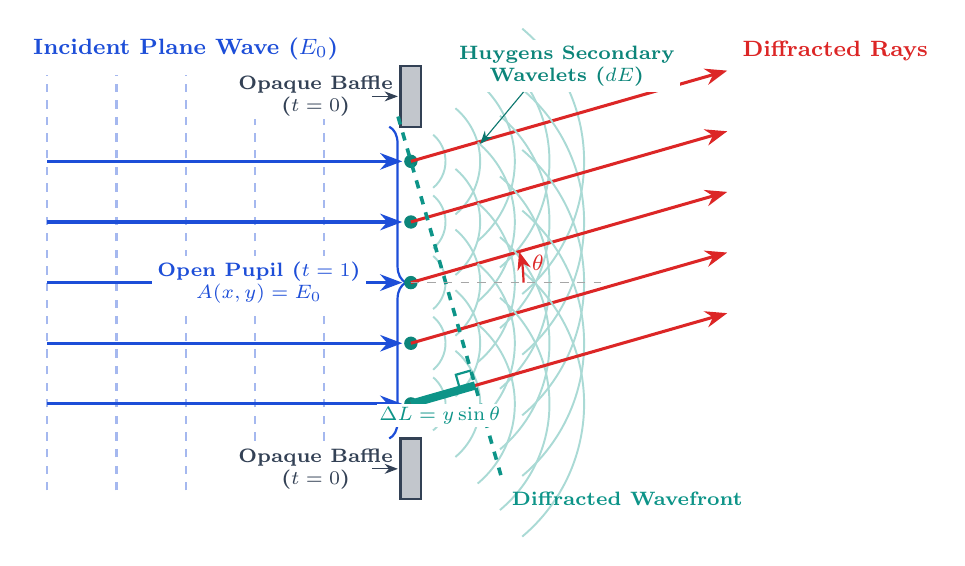
\begin{tikzpicture}[scale=1.1, >=Stealth]
    % Coordinates & parameters
    \def\apertureTop{1.8}
    \def\apertureBot{-1.8}
    \def\thetaDeg{16}
    \def\rayLen{3.8}
    
    % Colors
    \definecolor{incidentCol}{HTML}{1D4ED8}
    \definecolor{waveletCol}{HTML}{0D9488}
    \definecolor{rayCol}{HTML}{DC2626}
    \definecolor{opaqueCol}{HTML}{334155}
    
    % 1. Incident Plane Wave from Distant Star (Left)
    \foreach \x in {-4.2, -3.4, -2.6, -1.8, -1.0} {
        \draw[thick, incidentCol!40, dashed] (\x, -2.4) -- (\x, 2.4);
    }
    \foreach \y in {-1.4, -0.7, 0, 0.7, 1.4} {
        \draw[->, line width=1.1pt, incidentCol] (-4.2, \y) -- (-0.1, \y);
    }
    \node[incidentCol, fill=white, inner sep=2pt, font=\bfseries\footnotesize, align=center] at (-2.6, 2.7) {Incident Plane Wave ($E_0$)};

    % 2. Aperture Mask Plane (x = 0)
    % Top opaque mask
    \fill[opaqueCol!30] (-0.12, \apertureTop) rectangle (0.12, 2.5);
    \draw[thick, opaqueCol] (-0.12, \apertureTop) rectangle (0.12, 2.5);
    \node[opaqueCol, font=\scriptsize\bfseries, align=center, fill=white, inner sep=1pt] at (-1.1, 2.15) {Opaque Baffle\\($t=0$)};
    \draw[->, thin, opaqueCol] (-0.45, 2.15) -- (-0.15, 2.15);

    % Bottom opaque mask
    \fill[opaqueCol!30] (-0.12, \apertureBot) rectangle (0.12, -2.5);
    \draw[thick, opaqueCol] (-0.12, \apertureBot) rectangle (0.12, -2.5);
    \node[opaqueCol, font=\scriptsize\bfseries, align=center, fill=white, inner sep=1pt] at (-1.1, -2.15) {Opaque Baffle\\($t=0$)};
    \draw[->, thin, opaqueCol] (-0.45, -2.15) -- (-0.15, -2.15);

    % Open Aperture Bracket
    \draw[decorate, decoration={brace, amplitude=6pt, mirror}, thick, incidentCol]
        (-0.25, \apertureBot) -- (-0.25, \apertureTop) 
        node[midway, left=8pt, fill=white, inner sep=2pt, font=\bfseries\scriptsize, align=center] {Open Pupil ($t=1$)\\$A(x,y) = E_0$};

    % 3. Huygens Point Sources & Secondary Wavelets
    \foreach \y [count=\idx] in {1.4, 0.7, 0, -0.7, -1.4} {
        \coordinate (H\idx) at (0, \y);
        \fill[waveletCol!90!black] (H\idx) circle (2.2pt);
        
        \foreach \r in {0.4, 0.8, 1.2, 1.6, 2.0} {
            \draw[waveletCol!35, line width=0.7pt] (H\idx) ++(-50:\r) arc (-50:50:\r);
        }
        
        \draw[->, line width=1.1pt, rayCol] (H\idx) -- ++(\thetaDeg:\rayLen);
    }
    
    \node[waveletCol!90!black, fill=white, inner sep=2pt, font=\bfseries\scriptsize, align=center] at (1.8, 2.5) {Huygens Secondary\\Wavelets ($dE$)};
    \draw[->, thin, waveletCol!80!black] (1.3, 2.2) -- (0.8, 1.6);

    % 4. Perpendicular Diffracted Wavefront & Path Differences
    \coordinate (Wtop) at (H1);
    \pgfmathsetmacro{\xDelay}{2.8*sin(\thetaDeg)*cos(\thetaDeg)}
    \pgfmathsetmacro{\yDelay}{-1.4 + 2.8*sin(\thetaDeg)*sin(\thetaDeg)}
    \coordinate (Wbot) at (\xDelay, \yDelay);
    
    \draw[dashed, line width=1.3pt, waveletCol] ($(Wtop)!-0.2!(Wbot)$) -- ($(Wtop)!1.4!(Wbot)$) 
        node[below right=2pt and 0pt, font=\bfseries\scriptsize, waveletCol] {Diffracted Wavefront};
    
    \draw[line width=3.0pt, waveletCol] (H5) -- (Wbot);
    \node[waveletCol, font=\bfseries\scriptsize, below=3pt, fill=white, inner sep=1pt] at ($(H5)!0.45!(Wbot)$) {$\Delta L = y\sin\theta$};

    \pgfmathsetmacro{\sq}{0.18}
    \draw[thick, waveletCol] 
        ($(Wbot) + ({-\sq*cos(\thetaDeg)}, {-\sq*sin(\thetaDeg)})$) -- 
        ++({-\sq*sin(\thetaDeg)}, {\sq*cos(\thetaDeg)}) -- 
        ($(Wbot) + ({-\sq*sin(\thetaDeg)}, {\sq*cos(\thetaDeg)})$);

    \draw[dashed, gray!70] (H3) -- ++(2.2, 0);
    \draw[->, thick, rayCol] (1.3, 0) arc (0:\thetaDeg:1.3);
    \node[rayCol, font=\footnotesize\bfseries, right] at ({1.3*cos(0.5*\thetaDeg)}, {1.3*sin(0.5*\thetaDeg)+0.05}) {$\theta$};

    \node[rayCol, font=\bfseries\footnotesize, above right=0pt and 2pt] at ({\rayLen*cos(\thetaDeg)}, {1.4 + \rayLen*sin(\thetaDeg)}) {Diffracted Rays};
\end{tikzpicture}
\end{document}
